\documentclass{report}
\usepackage{inputenc} 
\usepackage{graphicx}
\usepackage{caption}
\usepackage{float}


\title{Manual for setting up the sensors of the Monitoring Box}
\author{Mick Nieman \\ Amsterdam University of Applied Sciences \and Pjotr Scholtze \\ Amsterdam University of Applied Sciences \and Heeyeon Joung \\ Seoul National University of Science and Technolgy}
\date{November 2017}

\begin{document}
\maketitle

\tableofcontents

\chapter{Requirements}
For every sensor added there is need for an Arduino Nano. The Arduino Nano is a programmable microprocessor. Advanced users may be able to connect multiple sensors to a single Arduino Nano, note that this requires advanced knowledge of the communication protocols between the Raspberry Pi 3 b+ and Arduino Nano. Along with every Arduino Nano you need an USB A to Mini-USB B cable.  \\

The first item needed for the GPS sensor is the Global Positioning System (GPS) module. We have used the Digilent 410-237 GPS-receiver board. \\

For the temperature and humidity sensor we have used the DHT22 module, this is a digital temperature- and humidity sensor. the DHT22 is more accurate (0,5$^o$ accuracy) than the previous, DHT11. It has a temperature reach from -40 to +80 $^o$C. and has a humidity reach from 10\% to 90\% with an accuracy of 2,0 \%.  \\

The heart rate sensor consists of the MAXREFDES117\# Reference Design Board with optical heart rate and pulse-oximetry monitor. It has integrated Red and Infrared LEDs. This works best on a person's fingertip or earlobe. \\

The CO$_2$ sensor comes in two varieties, the regular sensor which is affordable but less accurate and the advanced which has a higher costs and comes with higher accuracy. \\
The 'Regular CO$_2$ sensor' uses the MIKROE-1630 Daughter Board from Air Quality Click. It's an MQ-135 High sensitivity air quality sensor and potentiometer. \\
The 'Advanced CO$_2$ sensor' uses the K-30 CO$_2$ Engine from SenseAir. The K-30 sensor is an accurate gas sensor sensing up to 5000ppm (CO$_2$) with an accuracy of 3\%. Note that the advanced CO$_2$ meter does not work on the Arduino Nano and is only tested on the Arduino Uno. \\

The raspberry Pi Cam doesn't require to be connected to an Arduino and can be plugged directly in to the Raspberry Pi its camera-port. For this project we used Sony's IMX219 8-Megapixel Pi Camera Board. It is able for taking photographs of 3280x2464 pixels or video's at 1080p at 30 frames per second. \\

The galvanic skin response sensor, or short GSR, measures the galvanic skin response based on the electrical conductance of the skin. For the Monitoring Box we have used the Grove-GSR sensor from seeed studio.\\

Every sensor has it's own schematics for assembling the sensors, the code running on the sensor can be downloaded from https://github.com/pjotrscholtze/MonitoringBox, for the exact link for a particular sensor see further into this document.  \\

For the sake of easy searching there's all of the used materials listed below.\\

Always needed:

\begin{itemize}
\item Arduino Nano (ATMega 328 or better)
\item USB A to Mini-USB B cable
\item Arduino connector wires
\item Raspberry Pi 3 model b
\item Micro SD card (4GB minimum, 16GB or more advised)
\item Micro USB power supply (2.1A)
\item Digilent 410-237 GPS-receiver Board as the Global Positioning System module
\end{itemize}

Depending on your wishes you can use one or more of the following sensors:
 
\begin{itemize}
\item The DHT22 module for temperature and humidity
\item The MAXREFDES117\# Reference Design Board with optical heart rate and pulse-oximetry as a heart rate sensor
\item Regular CO2 sensor: MIKROE-1630 Daughter board from Air Quality Click. 
\item Advanced CO2 sensor: Senseair K-30 CO2 Engine.
\begin{itemize}
\item When using the Advanced CO2 sensor also an Arduino UNO board (ATMega328 or better) is needed along with an USB A to USB B cable 
\end{itemize} 
\item Raspberry Pi camera-module Camera V2 8MP (Sony IMX219) with CSI-interface cable
\item Grove-GSR from seeed studio for Galvanic Skin Response measurements
\end{itemize}

\chapter{Glossary}
\begin{tabular}{p{4,5cm} p{4,5cm}}
A & A \\
Ax Pin & Pin on arduino that is giving analog output \\
Arduino Nano & Programmable microprocessor, processes simple code \\
Arduino UNO & Programmable microprocessor, processes simple code \\
G & G \\
Galvanic Skin Response & The conductance of the skin that is being measured by its galvanic values \\
GND Pin & The pin that functions as 'ground' on an Arduino\\
H & H \\
Hardware & The machines, wiring, and other physical components of an electronic system \\
I & i \\
IDE & Integrated Development Environment, production supplied development environment \\
P & p \\
Protocol & Used by machines to communicate \\
R & R \\
Raspberry Pi & Advanced programmable processor, similar to Arduino but better \\
S & S \\
Software & Code on a processor or machine that defines behaviour\\
\end{tabular}

\chapter{Global Positioning System (GPS) sensor}
The Global Positioning System(GPS) sensor, from now on called the GPS sensor, is named PmodGPS. The schematics for the assembly of the sensor are as follows. \\

\begin{figure}[H]
\begin{center}
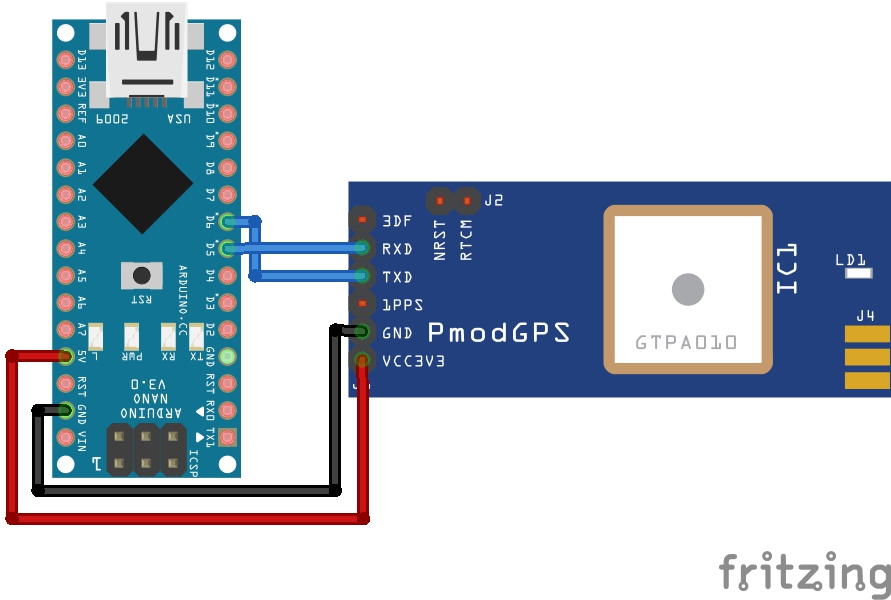
\includegraphics[scale=1]{images/GPS.jpg}
\caption{Global Positioning System Schematics}	
\end{center}
\end{figure}
\newpage
Below is the picture of the PmodGPS: \\

\begin{figure}[H]
\begin{center}
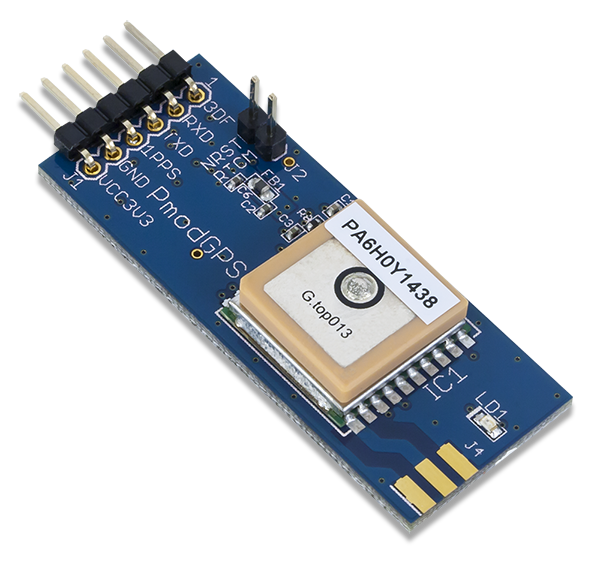
\includegraphics[scale=1]{images/GPSsensor.png}
\caption{GPS sensor}
\end{center}
\end{figure}


\begin{itemize}
\item 'VCC3V3' of the GPS sensor goes to the 5V(or VCC) of the Arduino, 
\item 'GND' of the GPS sensor goes to the GND of the Arduino,
\item 'RXD' of the GPS sensor goes to D5 pin(TXD) of the Arduino 
\item 'TXD' of the GPS sensor goes to D6 pin(RXD) of the Arduino. 
\end{itemize}

The code coming with this sensor can be downloaded with the following link: $ MonitoringBox/Sensor\_driver/main\_GPS\_SENSOR $


Downloading the code and uploading this to the Arduino Nano, see chapter 'Pushing code to an Arduino Nano', and having it assembled as the schematics show should result in a functional sensor. 





\chapter{Temperature and humidity sensor}
The Temperature and humidity sensor is named 'DHT22' and 'AM2302'. The schematics for the assembly of the sensor are as follows.\\

\begin{figure}[H]
\begin{center}
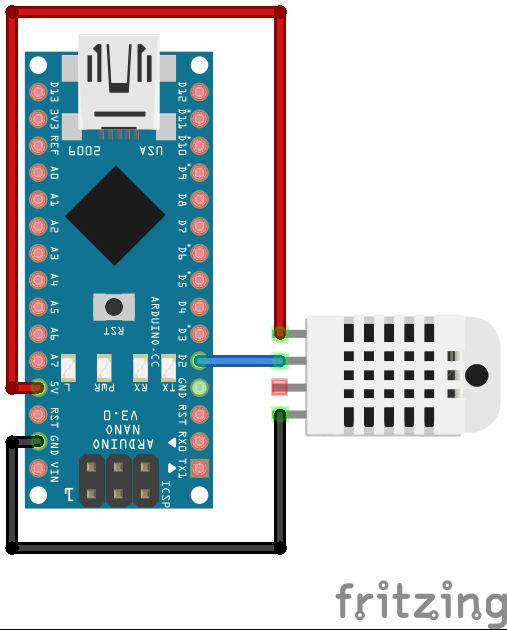
\includegraphics[scale=1.25]{images/H&T.jpg}
\caption{Temperature and humidity Schematics}	
\end{center}
\end{figure}
\newpage
Below is the picture of explaining pin on the DHT22 \\

\begin{figure}[H]
\begin{center}
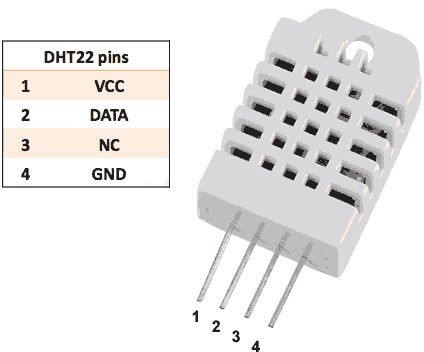
\includegraphics[scale=0.25]{images/DHT22.jpg}
\caption{Temperature and humidity sensor}
\end{center}
\end{figure}


There is no pin name on the sensor, so you need to see the order in which the pins are listed. When looking at the sensor in front, I'll call the leftmost pin 'pin1'.\\

\begin{itemize}
\item 'pin 1' of the Temperature and humidity sensor(VCC) goes to the 5V(or VCC) of the Arduino, 
\item 'pin 2' of the Temperature and humidity sensor(DATA) goes to the D2 of the Arduino,
\item 'pin 3' of the Temperature and humidity sensor is nothing. You do not need to connect anything.
\item 'pin 4' of the Temperature and humidity sensor(GND) goes to GND of the Arduino.
\end{itemize}
 
The code coming with this sensor can be downloaded with the following link: $ MonitoringBox/Sensor\_driver/main\_TEM\_AND\_HUM\_SENSOR $


Downloading the code and uploading this to the Arduino Nano, see chapter 'Pushing code to an Arduino Nano', and having it assembled as the schematics show should result in a functional sensor. 


\chapter{Heartrate sensor}
The Heart-rate sensor which is a sensor developed by Maxim intergrated is named MAXREFDES117\#. The schematics for the assembly of the sensor are as follows.\\

\begin{figure}[H]
\begin{center}
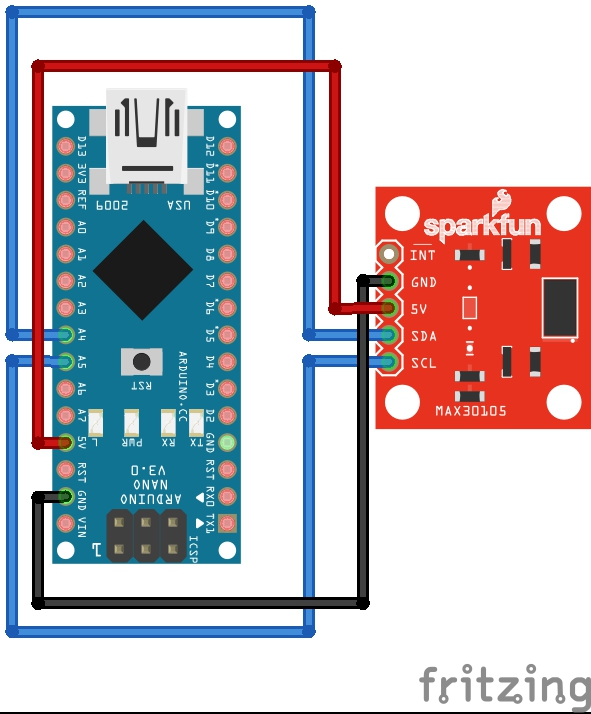
\includegraphics[scale=1.25]{images/heartrate_bb.jpg}
\caption{Heart rate Schematic}
\end{center}
\end{figure}

Note that the actual sensor looks quite different, though the pinout is the same.\\

The actual sensor looks like the following:\\

\begin{figure}[H]
\begin{center}
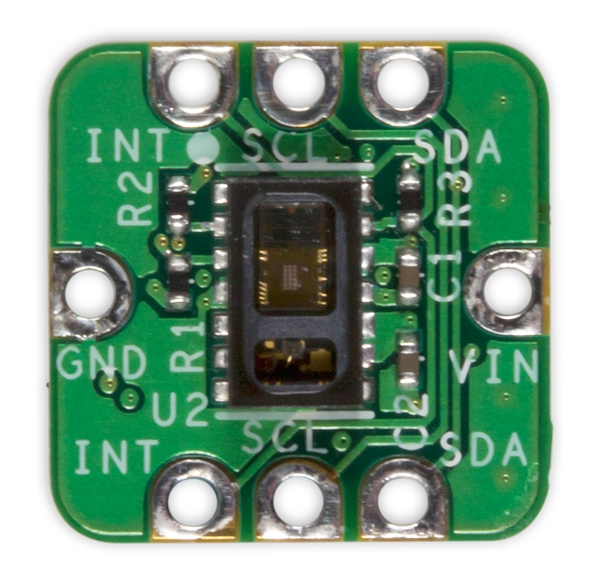
\includegraphics[scale=0.25]{images/MAXREFDES117Fig00.png}
\caption{Heart rate sensor}
\end{center}
\end{figure}

\begin{itemize}
\item 'VIN' of the Heartrate sensor goes to the 5V(or VCC) of the Arduino, 
\item 'GND' of the Heartrate sensor goes to the GND of the Arduino,
\item 'SDA' of the Heartrate sensor goes to A4 pin(SDA) of the Arduino 
\item 'SCL' of the Heartrate sensor goes to A5 pin(SCL) of the Arduino.\\
\\In Arduino-nano that we used doesn't have SDA and SCL name on the arduino. However, A4 and A5 act as SDA and SCL, respectively. If your Arduino has an SDA or SCL pin, you can connect it by name.
 
\end{itemize}
The code coming with this sensor can be downloaded with the following link: $ MonitoringBox/Sensor\_driver/main\_HEARTRATE\_SENSOR $


Downloading the code and uploading this to the Arduino Nano, see chapter 'Pushing code to an Arduino Nano', and having it assembled as the schematics show should result in a functional sensor. \\
For more information about this sensor, Please visit below website.\\
https://www.maximintegrated.com/en/design/reference-design-center/system-board/6300.html



\chapter{Regular carbon dioxide (CO$_2$) sensor}
The regular carbon dioxide (CO$_2$) sensor, from now on called the regular (CO$_2$) sensor, is a sensor developed by mikroelectronics, and the schematics for the assembly of the sensor are as follows. \\

\begin{figure}[H]
	\centering
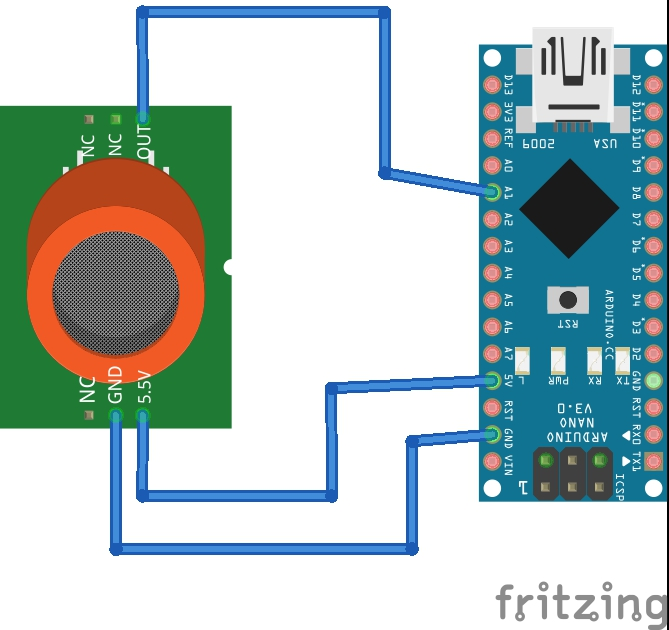
\includegraphics[width=0.75\textwidth]{images/Mikroe-Gas-sensor-schematic.jpg}
	\caption{Air Quality Click Schematic}
\end{figure}

Note that the actual sensor looks slightly different, though the pinout is the same, the 5.5V pin of the Air-quality-click goes onto the 5.5V pin on the Arduino, the GND pin on the Air-quality-click  goes onto the GND pin on the Arduino and the OUT pin on the Air-quality-click goes onto the A1 pin of the Arduino. \\
The actual sensor looks like the following:\\

\begin{figure}[H]
	\centering
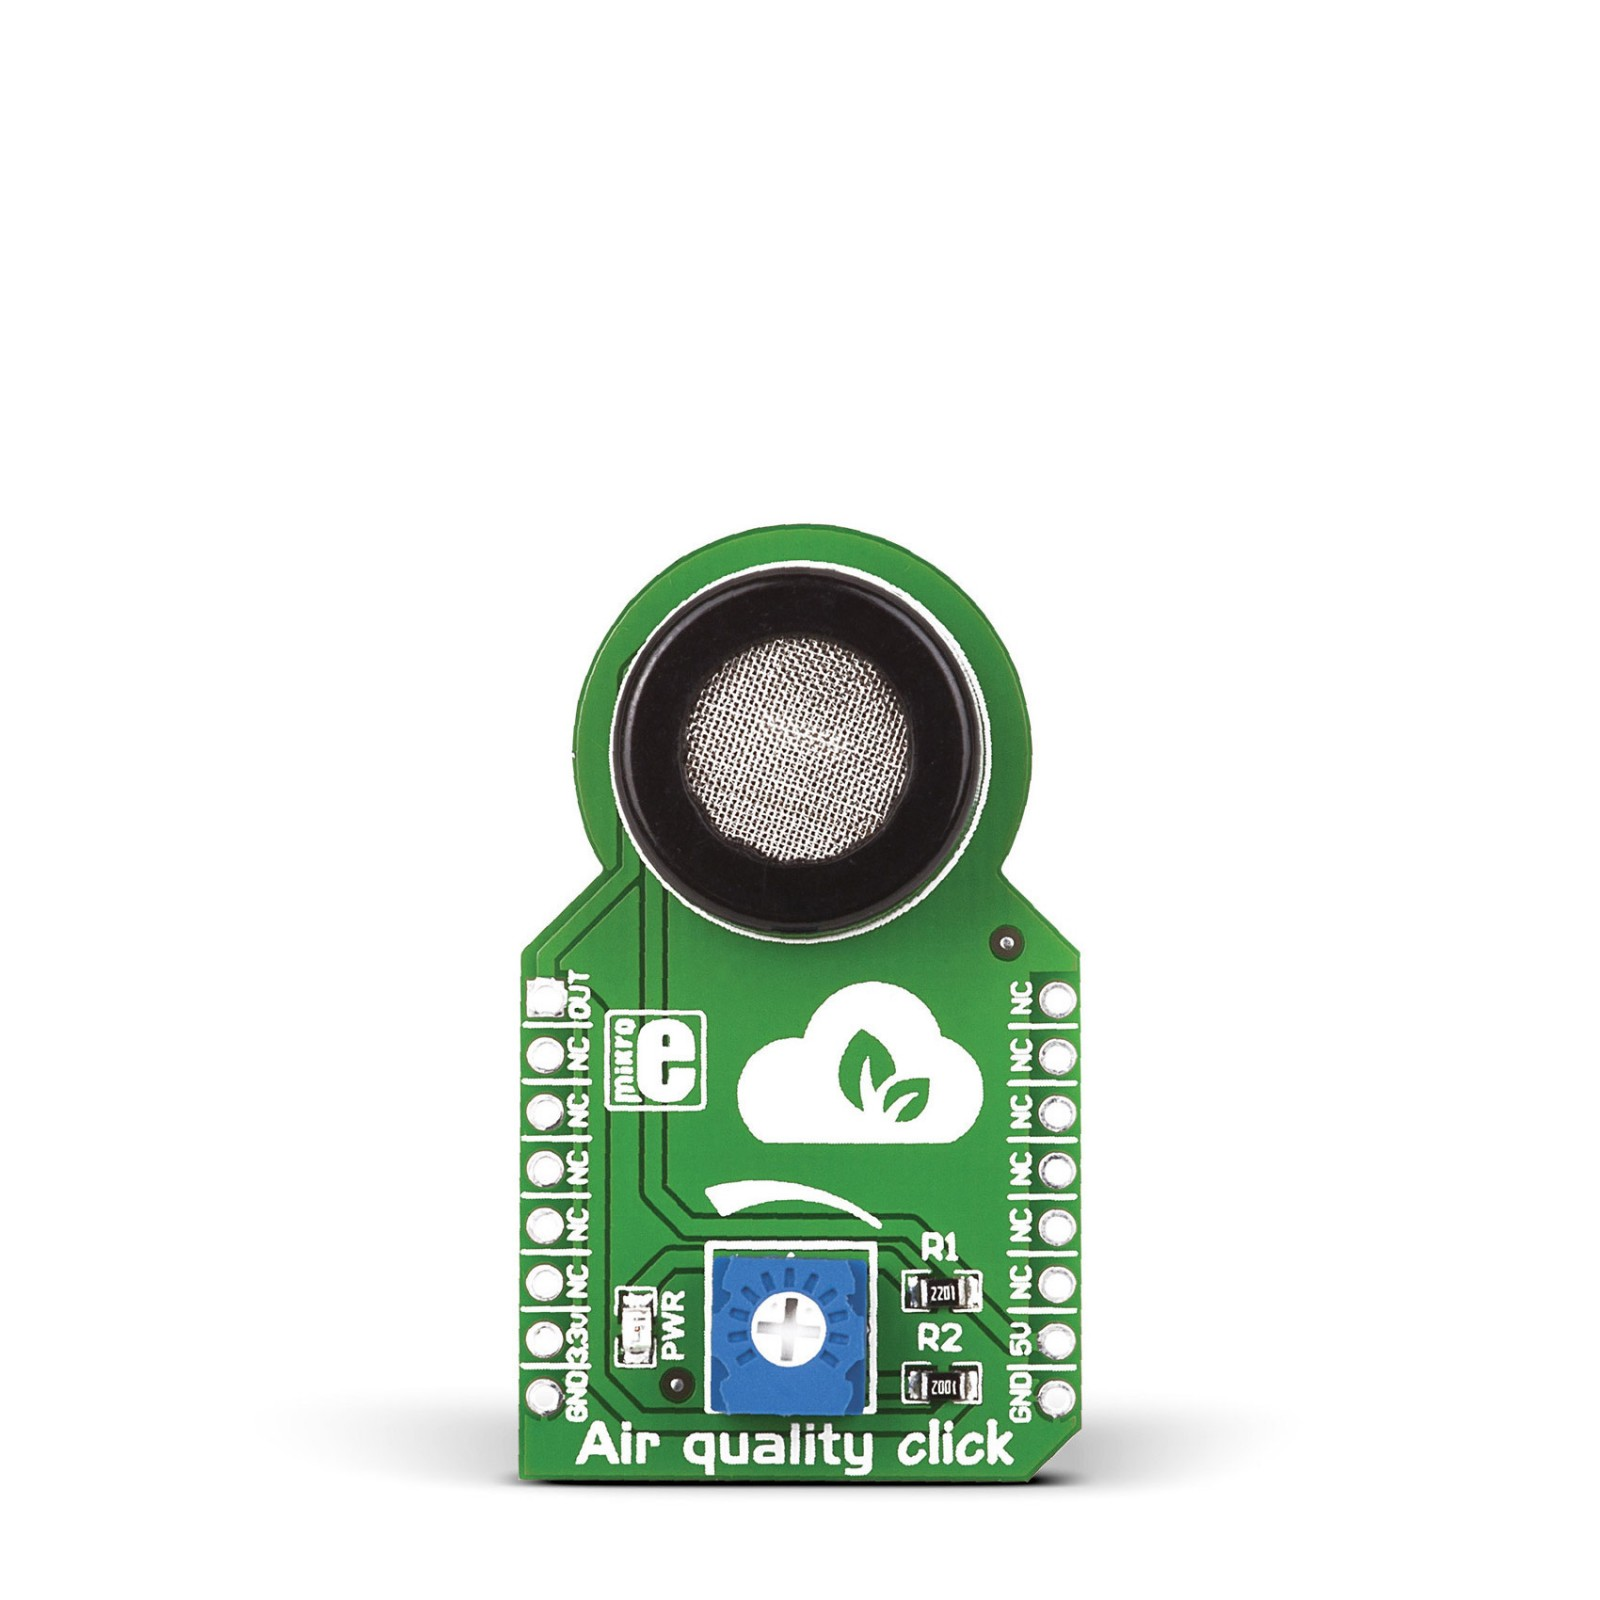
\includegraphics[width=0.75\textwidth]{images/air-quality-click-breakout.jpg} 
	\caption{The Mikroe Gas Detector}
\end{figure}

The code coming with this sensor can be downloaded with the following link: $ https://github.com/pjotrscholtze/MonitoringBox/tree/develop/Sensors/CO2\_Sensor $


Downloading the code and uploading this to the Arduino Nano, see chapter 'Pushing code to an Arduino Nano', and having it assembled as the schematics show should result in a functional sensor. 

\chapter{Advanced carbon dioxide (CO$_2$) sensor}
For starters, this CO$_2$ sensor is a little bit more complex than the other CO$_2$ sensor from the previous chapter. This sensor is more accurate but also works in a different way and not only the accuracy is higher, so is the price. 
The CO$_2$ sensor is developed by CO2meter.com and currently we're using the K30 model. During our testing phase we discovered that the K30 model is not compatible with the Arduino Nano nor with the Arduino Pro Mini but it is compatible with the Arduino UNO. 

\begin{figure}[H]
	\centering
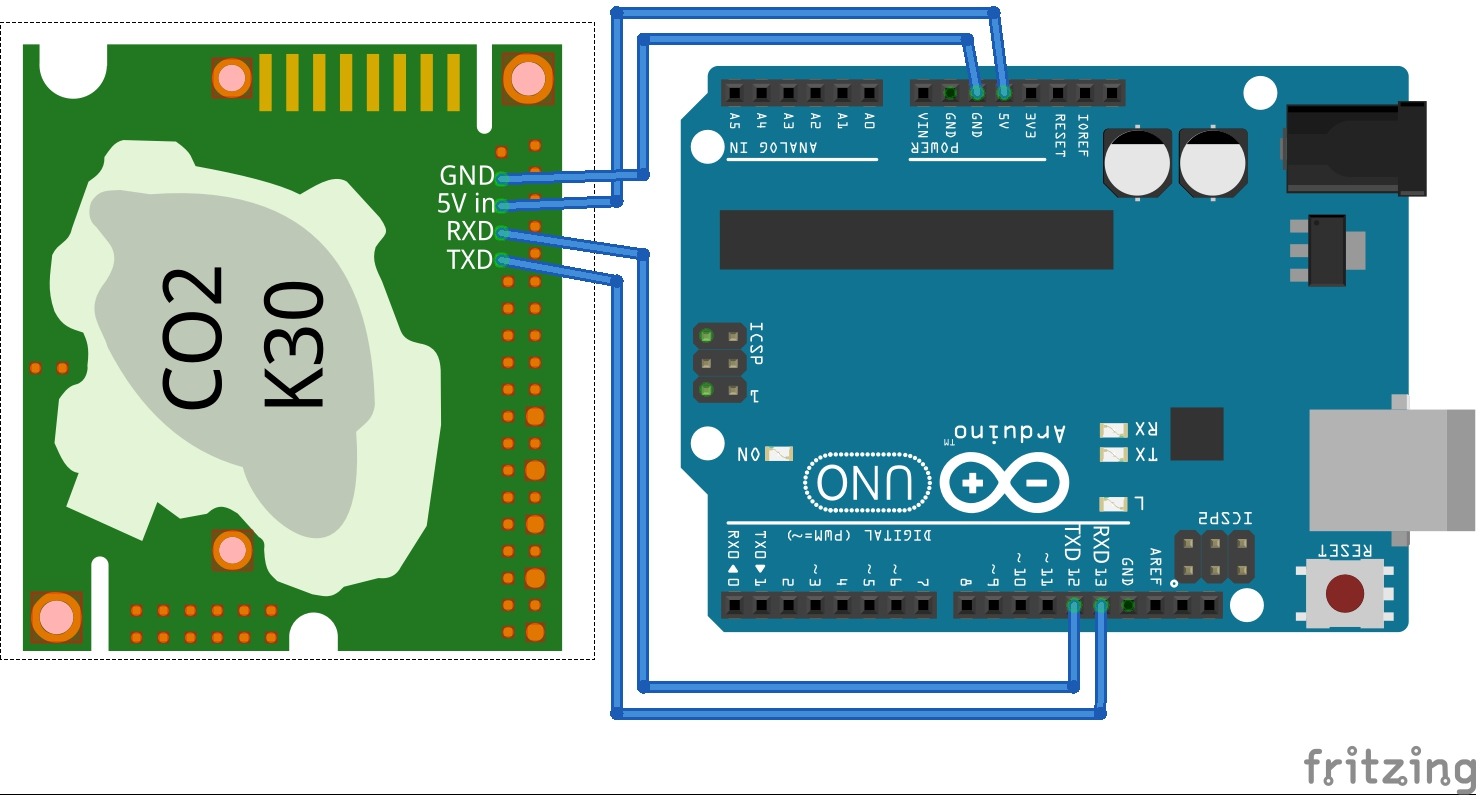
\includegraphics[width=0.75\textwidth]{images/K30-gas-sensor-schematic.jpg} 
	\caption{The K30 CO$_2$ sensor from  CO2meter.com}
\end{figure}

After assembling the pins the right way, note that the pins on the K30 aren't labeled, but you will have to attach them to the inner (second) row, skipping the first pin, so using pin 2, 3, 4 and 5 from right to left. 
\begin{itemize}
\item 'pin 2' of the K30 goes to the GND of the Arduino, 
\item 'pin 3' of the K30 goes to the 5V (or VCC) of the Arduino,
\item 'pin 4' (the RXD pin) of the K30 goes to pin 13 (TXD)of the Arduino 
\item 'pin 5' of the K30 (TXD) goes to pin 12 (RXD) of the Arduino. 

Downloading the code from https://github.com/pjotrscholtze/MonitoringBox and uploading the code to the Arduino UNO (this works the same way as with the Arduino Nano, see chapter 'Pushing code to an Arduino Nano') should result in a functional CO$_2$ sensor. 
\end{itemize}
\chapter{Raspberry Pi Camera}
\begin{figure}[H]
	\centering
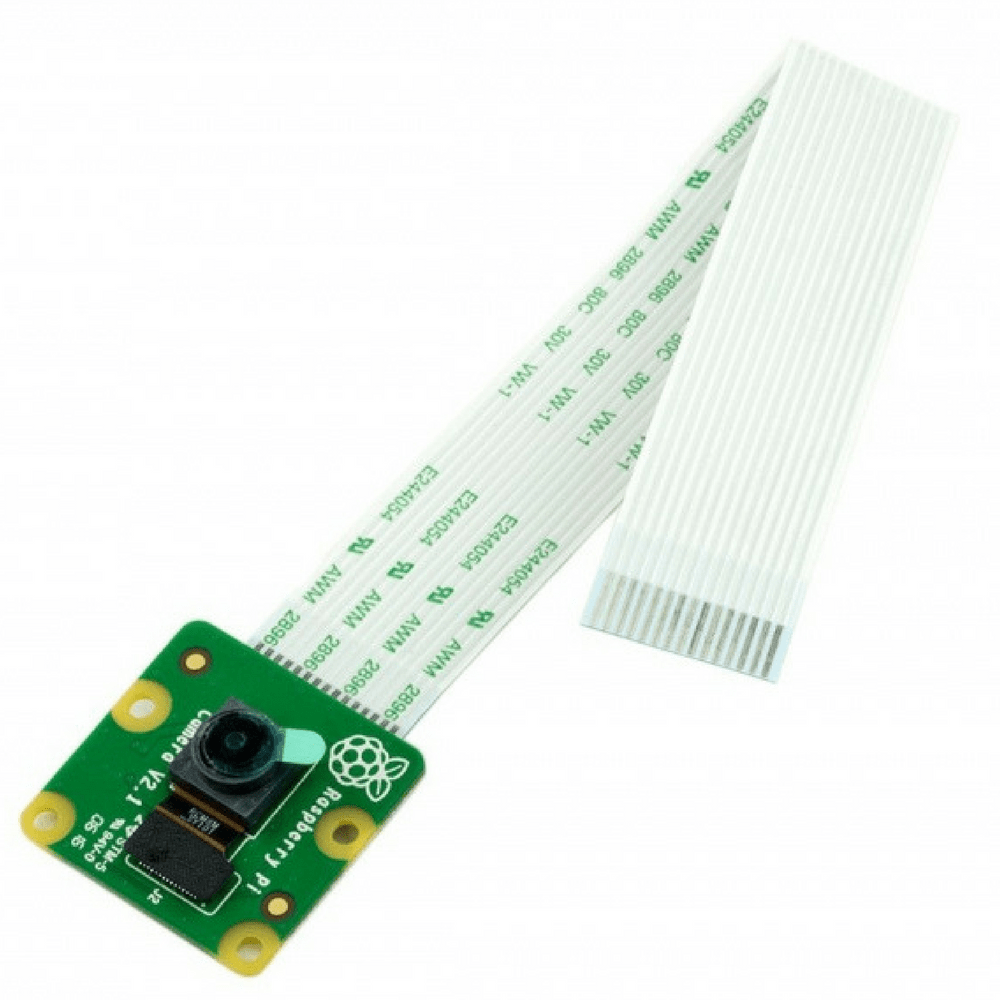
\includegraphics[width=0.50\textwidth]{images/Raspberry-Pi-Camera-Board-v2-1.png}
\caption{The Raspberry Pi Camera}	
\end{figure}

The raspberry Pi cam doesnt require any extra hardware as an Arduino, it can be directly plugged into the Raspberry Pi and it will be detected by the Raspberry Pi as a camera. \\
Do note that there are two similar connectors that the Camera may fit in, one is named 'Camera' and the other is named 'Display' connector. We will be using the 'Camera' connection. The next image shows the connector and the direction to pull in order to open it.  

\begin{figure}[H]
	\centering
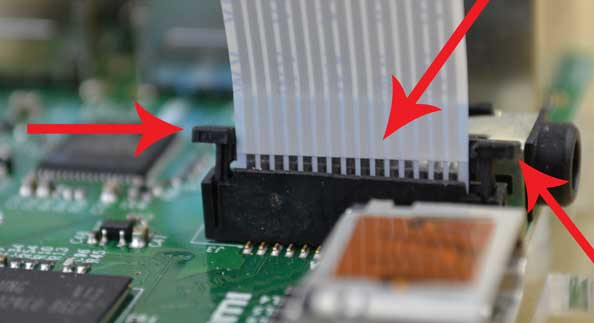
\includegraphics[width=0.50\textwidth]{images/clips-and-ribbon-cable.jpg}
\caption{The Raspberry Pi Camera connector}	
\end{figure}

Pull the connector lid on both sides of the connector in order to open, insert the Pi Camera and close the connector by pushing on both sides of the connector, as the arrows in the images implies. 

\chapter{Galvanic skin response sensor}
Galvanic skin response sensor(GSR) sensor, from now on called the GSR sensor, does not require any sensor hardware. Only a little resistance is needed for stability. There a free choice for the type of resistor , but a resistor with less than 1k resistance is recommended. The schematics for the assembly of the sensor are as follows. \\

\begin{figure}[H]
\begin{center}
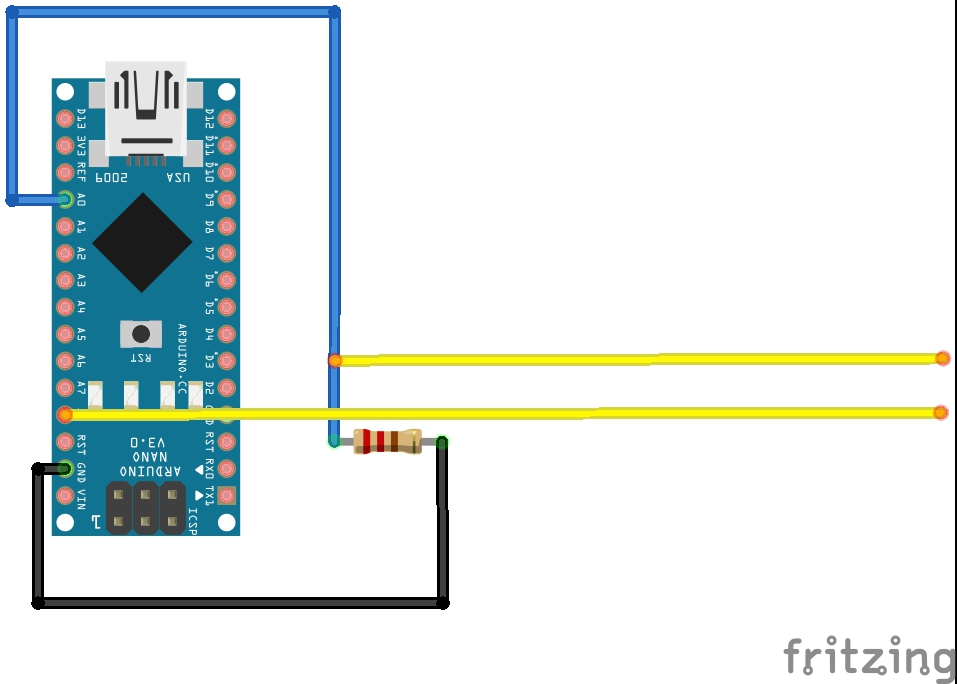
\includegraphics[scale=1.25]{images/GSR.jpg}
\caption{Galvanic skin response Schematic}
\end{center}
\end{figure}

The two current-carrying wires are connected to A0 and 5V, respectively, of the Arduino. The resistors for stability are connected to A0 and GND respectively.	\\

The code coming with this sensor can be downloaded with the following link: $ MonitoringBox/Sensor\_driver/main\_GSR\_SENSOR $


Downloading the code and uploading this to the Arduino Nano, see chapter 'Pushing code to an Arduino Nano', and having it assembled as the schematics show should result in a functional sensor.\\

The way to use this GSR sensor is to put two fingers on two wires. Individual currents are different and will vary depending on emotional state or condition. To compare this, the result of the sensor will show the minimum, maximum and average values ​​of the current. An example of usage and the result value are shown in the following photograph.

\chapter{Pushing code to an Arduino Nano}
To start working with an Arduino the Arduino Integrated development environment (IDE) is needed. This is a development environment custom build by Arduino for the Arduino. The IDE can be retrieved from their site www.arduino.cc and the direct link to their software downloads is https://www.arduino.cc/en/Main/Software. Then download the right IDE for your operating system to continue. \\

Installing the software and then opening the program results in a screen similar to the next. 

\begin{figure}[H]
	\centering
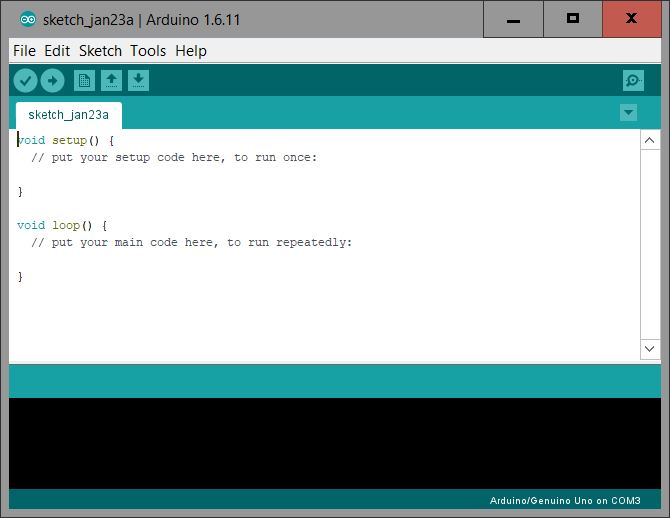
\includegraphics[width=1\textwidth]{images/ArduinoIDE.JPG} 
	\caption{Arduino IDE start screen}
\end{figure}

Putting code on the Arduino means either \\
a). Opening one of the pre-configured packages that came with the software of the Monitoring Box and start uploading or \\
b). Copying the code from your source to the Arduino IDE and then uploading the code. \newpage

Step 1. connecting the Arduino to your computer by using the USB cable. \\
Step 2. Opening the package containing the desired code for the Arduino. \\
Step 3. Selecting the right board as shown in the next figure. \\
\begin{figure}[H]
	\centering
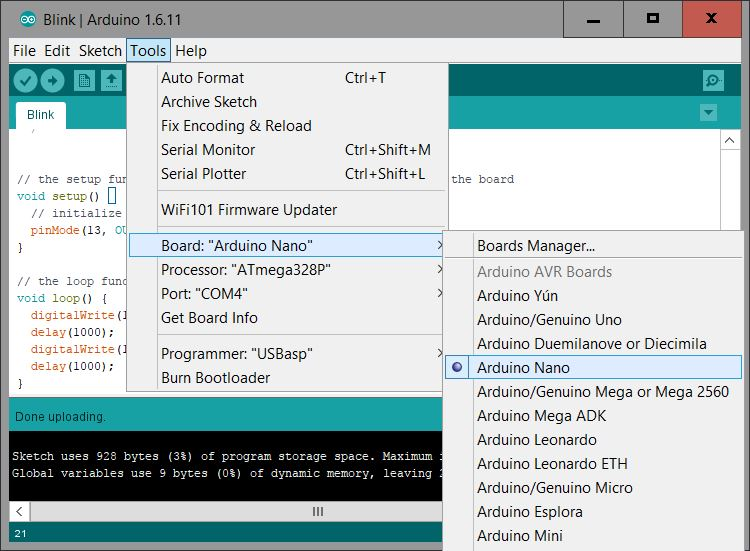
\includegraphics[width=1\textwidth]{images/Select-board.JPG} 
	\caption{Selection of the right board via Arduino IDE}
\end{figure}
\newpage
Step 4. Selecting the right port as shown in the next figure, the port may differ every time you connect. Usually the IDE only shows one port, select this one. \\
\begin{figure}[H]
	\centering
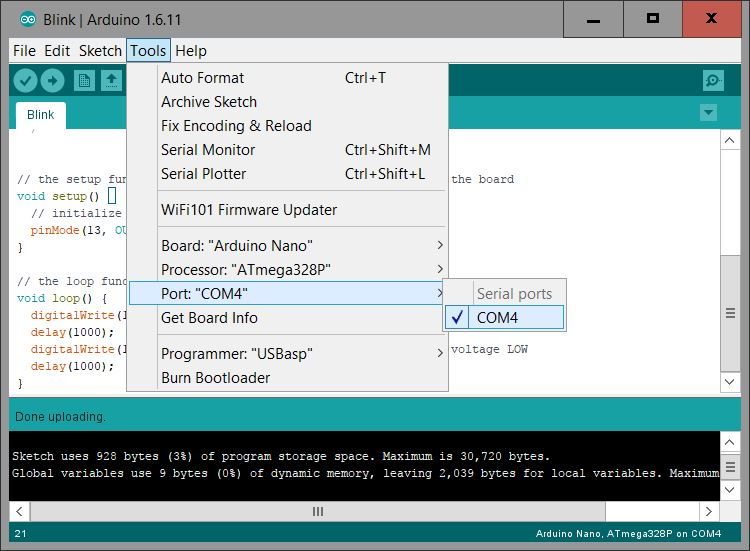
\includegraphics[width=1\textwidth]{images/Select-port.JPG} 
	\caption{Selection of the right port via Arduino IDE}
\end{figure}
Step 5. Verifying the code by pressing the 'verify button' (the check-mark). \\
Step 5.1 Failed verifying; start troubleshooting. \\
Step 5.2 Succeeded verifying; continue. \\
Step 6. Uploading the code to your Arduino by pressing the 'upload button' (the right-arrow). \\
Step 6.1 Failed verifying; start troubleshooting. \\
Step 6.2 Succeeded verifying; continue. \\
Step 7. Close program and disconnect the Arduino from your computer. \\

\end{document}
